\documentclass[a4paper, 12pt]{article}
\usepackage[portuguese,provide=*]{babel}
\usepackage[utf8]{inputenc}
\usepackage[T1]{fontenc}
\usepackage{times}
\usepackage{setspace}
\usepackage{mathptmx} 
\onehalfspacing
\usepackage{amsmath}
\usepackage{indentfirst}
\usepackage{graphicx}
\usepackage{multicol}
\usepackage{enumitem}
\usepackage{url}
\usepackage{booktabs}
\usepackage{array}
\usepackage{tocloft}
\usepackage{fancyhdr}
\usepackage{tabularx}   
\usepackage{longtable}
\usepackage{float}
\usepackage{booktabs}   
\usepackage{makecell}
\usepackage{xcolor}
\usepackage{hyperref}
\usepackage{amssymb}
\usepackage[a4paper, 
            left=3cm,    
            right=2cm,   
            top=3cm,    
            bottom=2cm   
            ]{geometry}

\begin{document}

\begin{titlepage}
	\begin{center}
	
	\begin{figure}[!ht]
	\centering
	  
\includegraphics[width=10cm]{dist/LogoTransparentePreto.png} \\ 
    \end{figure}

	\vspace{115pt}
    \textbf{\Huge{Projeto de Interface}}\\
        
	\vspace{115pt}
    Carlos Eduardo Nogueira Silva \\
    Felipe Gomes da Silva \\
    Felipe Matheus Possari \\
    Matheus Thomé da Silva\\ 
    Santiago Pinheiro Martins \\
	\end{center}
	
	\vspace{1cm}
	\begin{center}
		\vspace{\fill}
		Abril \\
		2025
	\end{center}
\end{titlepage}

\newpage
\thispagestyle{empty}
\tableofcontents

\newpage
\pagestyle{fancy}
\fancyhead[L]{\thepage}
\fancyhead[C]{\nouppercase{\leftmark}}
\rhead{
\includegraphics[width=2cm]{dist/LogoTransparentePreto.png}}
\fancyfoot[R]{}
\fancyfoot[C]{© 2025 - PuSystems}
\fancyfoot[L]{}
\setlength\headheight{26pt}

\section{Introdução}
A interface desempenha um papel essencial no sucesso do aplicativo, pois é o ponto de contato direto entre o usuário e as funcionalidades do sistema, sendo determinante para garantir a usabilidade, o engajamento e a eficácia das ações propostas. O objetivo central deste documento é detalhar o planejamento, o design e a construção das telas do sistema, com foco em criar uma experiência de usuário intuitiva, acessível e eficiente.

A interface foi desenvolvida levando em conta os princípios de usabilidade tradicionais, conforme Pressman \cite{pressman-2019} e Nielsen (1994), com o objetivo de satisfazer as demandas de diversos tipos de usuários, do mais iniciante ao mais avançado, minimizando falhas, diminuindo o esforço cognitivo e aprimorando a execução de tarefas. 
 
O documento descreve as etapas de análise, projeto, construção e validação, além de apresentar cada tela e suas respectivas decisões de design. O foco principal é garantir que a interface do aplicativo contribua efetivamente para engajar a população no combate à dengue, promovendo ações informadas e coletivas no contexto urbano de São José do Rio Preto.

\newpage
\section{Desenvolvimento}

\subsection{Análise}
A análise das interfaces do aplicativo Zapp foi realizada seguindo os princípios de usabilidade propostos por Pressman \cite{pressman-2019}, com o objetivo de assegurar que o design do sistema seja acessível, funcional e adaptável às necessidades reais dos usuários. Um aspecto crucial dessa análise foi a identificação minuciosa do perfil dos usuários, abrangendo desde pessoas iniciantes, que podem ter pouca experiência com tecnologia, até usuários intermediários e avançados, que necessitam de funcionalidades mais rápidas e eficazes.

Outro ponto examinado foram as tarefas que os usuários precisam executar no sistema. Isso engloba ações como login, registro, denúncia de focos, acompanhamento de sintomas, consulta a rankings e acesso a materiais educativos. Cada tarefa foi avaliada com base na frequência, complexidade e relevância, possibilitando a identificação de áreas críticas que necessitam de um cuidado especial no design. Por exemplo, diminuir a quantidade de cliques necessários para denúncias ou fornecer atalhos para funções mais usadas, o que aumenta a eficácia geral.

Adicionalmente, levou-se em conta o contexto físico de utilização do aplicativo, considerando que muitos usuários o usarão em locais públicos, ruas, com variações de luminosidade, e possivelmente enquanto desempenham outras tarefas (como caminhar ou conversar). Essa avaliação destacou a importância de desenvolver telas responsivas, com contraste apropriado, elementos grandes e bem dispostos, prevenindo o excesso de informação na tela ou solicitando interações excessivamente precisas que poderiam não funcionar em situações de movimento.

Finalmente, a análise considerou aspectos humanos cruciais, como a limitação da memória de curto prazo e a tendência inata de cometer erros. O sistema foi concebido para não sobrecarregar o usuário com informações demasiadamente complexas em uma única tela, além de oferecer suporte contínuo durante a interação, através de mensagens de confirmação, indicadores visuais claros e opções de recuperação de falhas. Esses componentes são cruciais para assegurar uma experiência não só funcional, mas também segura e confortável, fomentando a confiança no uso contínuo do aplicativo.

\subsection{Projeto}
O desenvolvimento das interfaces do aplicativo Zapp foi realizado cuidadosamente, levando em conta os princípios tradicionais de usabilidade e design focado no usuário.  Cada tela foi concebida não somente para desempenhar seu papel prático, mas também para proporcionar uma experiência fluida, intuitiva e eficaz, minimizando falhas, potencializando o envolvimento e assegurando a acessibilidade para diversos tipos de usuários.

\subsubsection{Tela de Login}

\begin{figure}[H]
  \centering
  \fbox{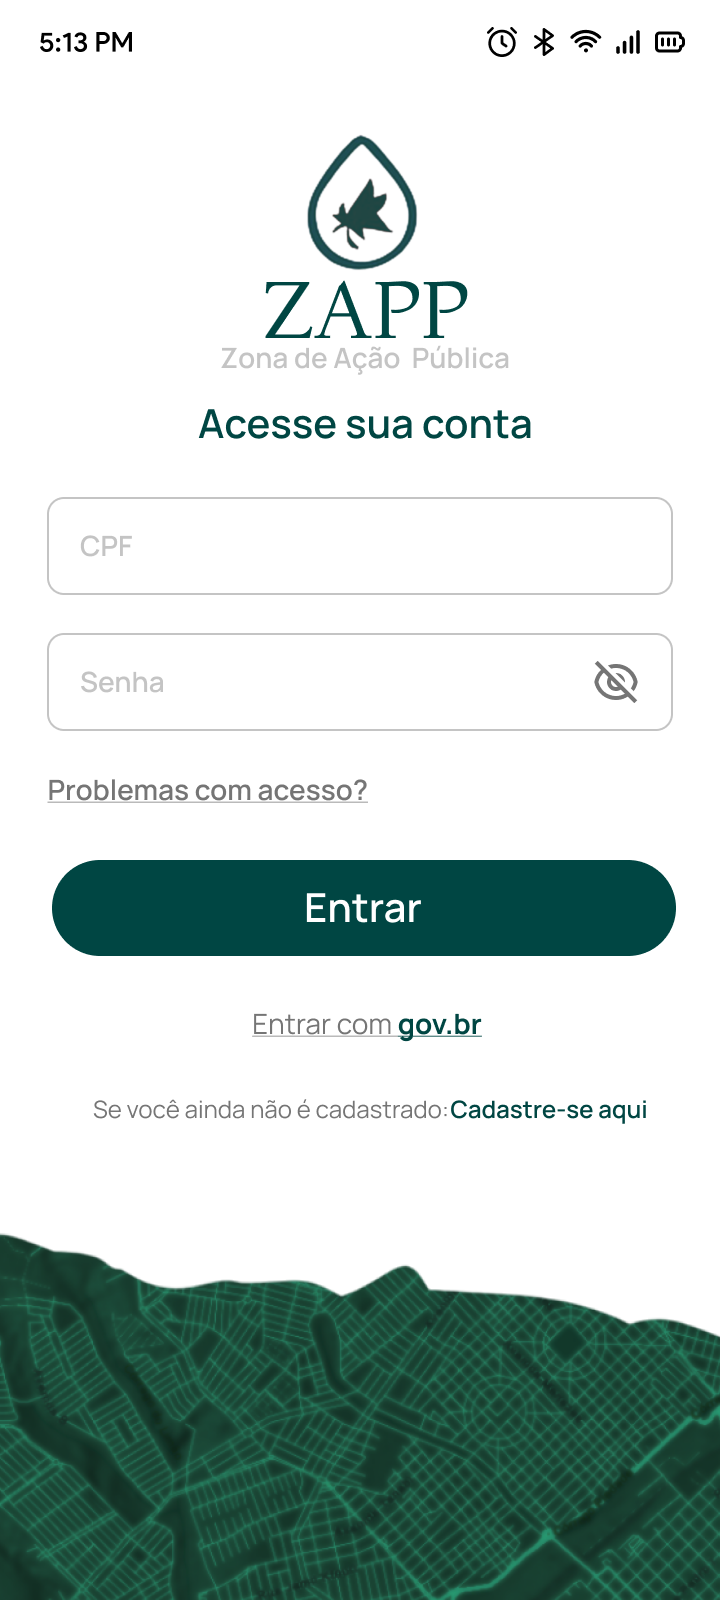
\includegraphics[width=0.5\textwidth]{dist/sign-in.png}}
  \caption{Tela de Login}
  \label{fig:login}
\end{figure}

No menu de login, optou-se por colocar o usuário no controle, proporcionando a flexibilidade entre o login convencional e a autenticação integrada ao sistema do gov.br.  Esta decisão possibilita ao usuário selecionar a alternativa que julga mais conveniente e segura, fortalecendo a sensação de controle.  Adicionalmente, foi adicionada a opção de recuperação de acesso para reduzir o efeito de senhas perdidas, prevenindo bloqueios desnecessários.  Itens minúsculos, como o ícone de olho que permite exibir ou esconder a senha, reforçam a confiança e a transparência. Por outro lado, o mapa localizado na parte inferior liga a identidade visual do aplicativo à proposta comunitária, intensificando o engajamento.

\subsubsection{Tela de Cadastro}

\begin{figure}[H]
  \centering
  \fbox{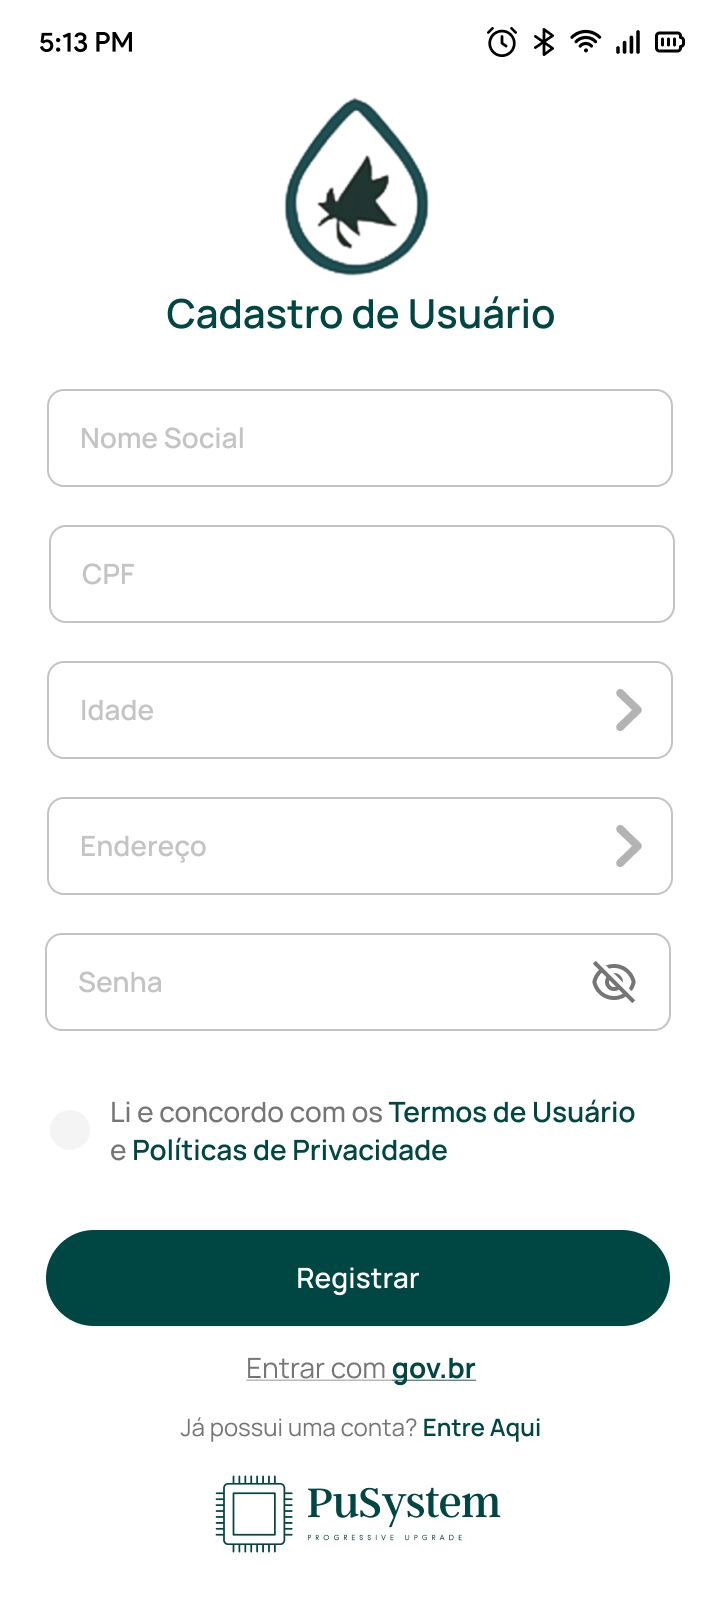
\includegraphics[width=0.5\textwidth]{dist/sign-up.png}}
  \caption{Tela de Cadastro}
  \label{fig:cadastro}
\end{figure}

A tela de cadastro segue essa mesma ideia da tela de login, com atenção a detalhes que melhoram a experiência do usuário. Incorporou-se a opção de autenticação alternativa pelo gov.br e uma separação visual evidente entre as alternativas para prevenir confusão.  Componentes como o link para os termos de uso e as políticas de privacidade fomentam a transparência e a responsabilidade. Por outro lado, a validação em tempo real dos campos e as orientações para a criação da senha direcionam o usuário e diminuem a possibilidade de falhas, tornando o procedimento mais seguro e eficaz.

\subsubsection{Home}

\begin{figure}[H]
  \centering
  \fbox{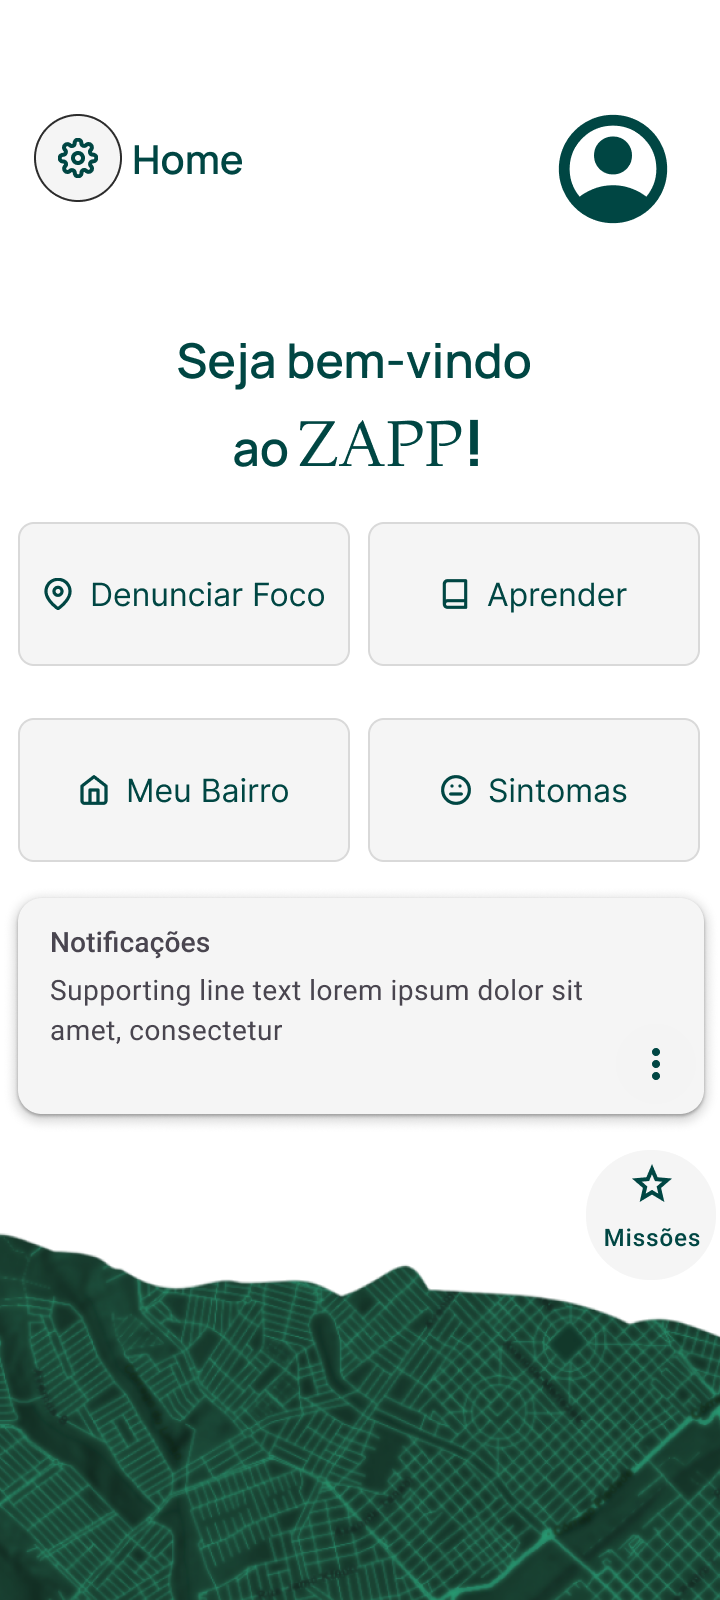
\includegraphics[width=0.5\textwidth]{dist/home.png}}
  \caption{Página Inicial}
  \label{fig:home}
\end{figure}

Na tela home, a navegação simplificada foi priorizada. Botões principais destacados e ícones autoexplicativos permitem acesso rápido às funções essenciais, enquanto áreas dedicadas para notificações e missões mantêm o usuário informado e engajado. Isso garante que as ações mais importantes estejam sempre visíveis, mesmo para usuários com pouca familiaridade tecnológica.

\subsubsection{Tela Meu Bairro}

\begin{figure}[H]
  \centering
  \fbox{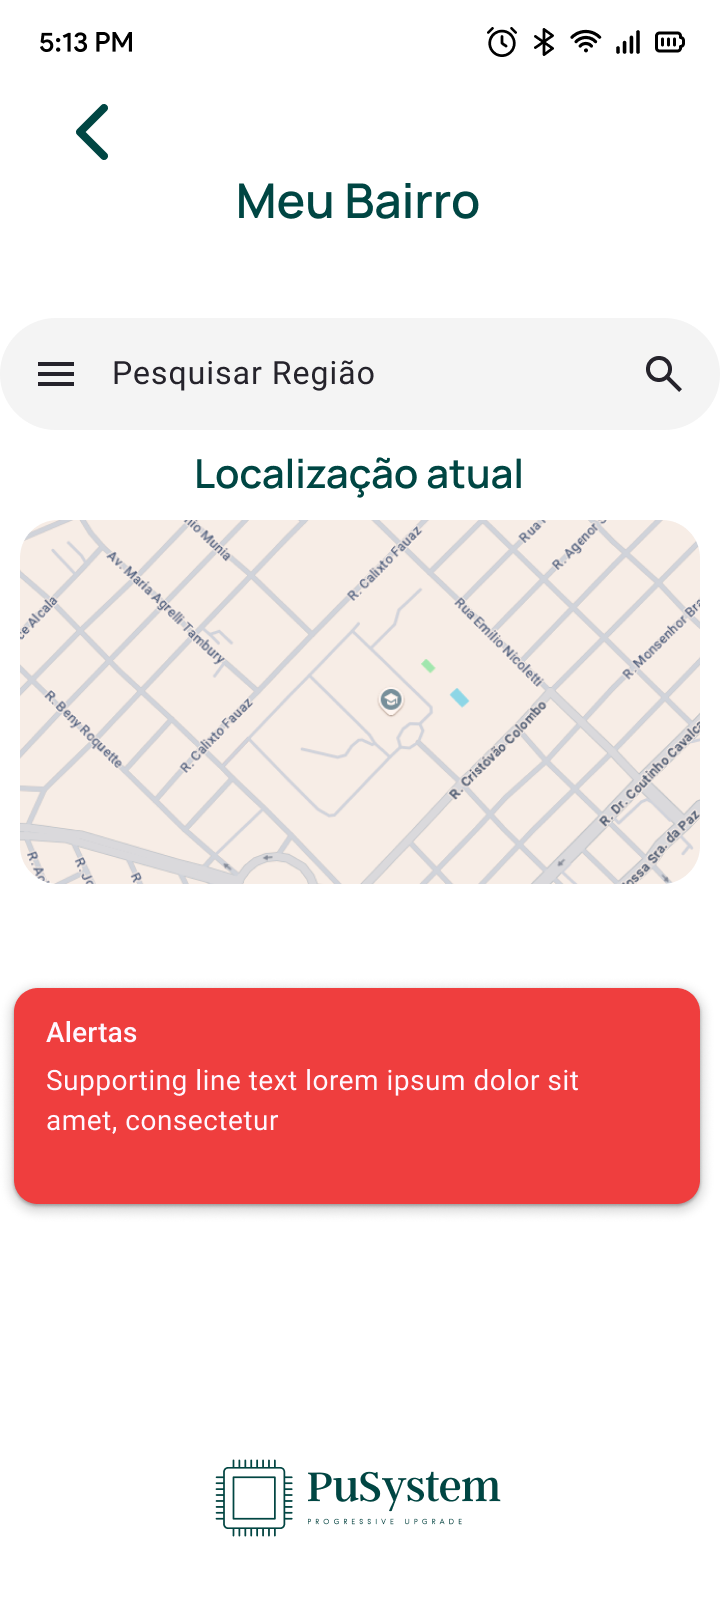
\includegraphics[width=0.5\textwidth]{dist/meu-bairro.png}}
  \caption{Mapa do Bairro Local}
  \label{fig:bairro}
\end{figure}

O "Meu Bairro" foi projetado para proporcionar uma orientação espacial eficiente.  O campo de busca por região e a relação de regiões próximas auxiliam o usuário na localização, enquanto uma seção dedicada a alertas oferece informações contextuais fundamentais para que ele entenda os riscos ao seu entorno.  O sistema de cores para priorização de alertas e o mapa interativo tornam a visualização mais intuitiva, possibilitando uma compreensão ágil e auxiliando na tomada de decisões.

\subsubsection{Tela Denunciar Foco}

\begin{figure}[H]
  \centering
  \fbox{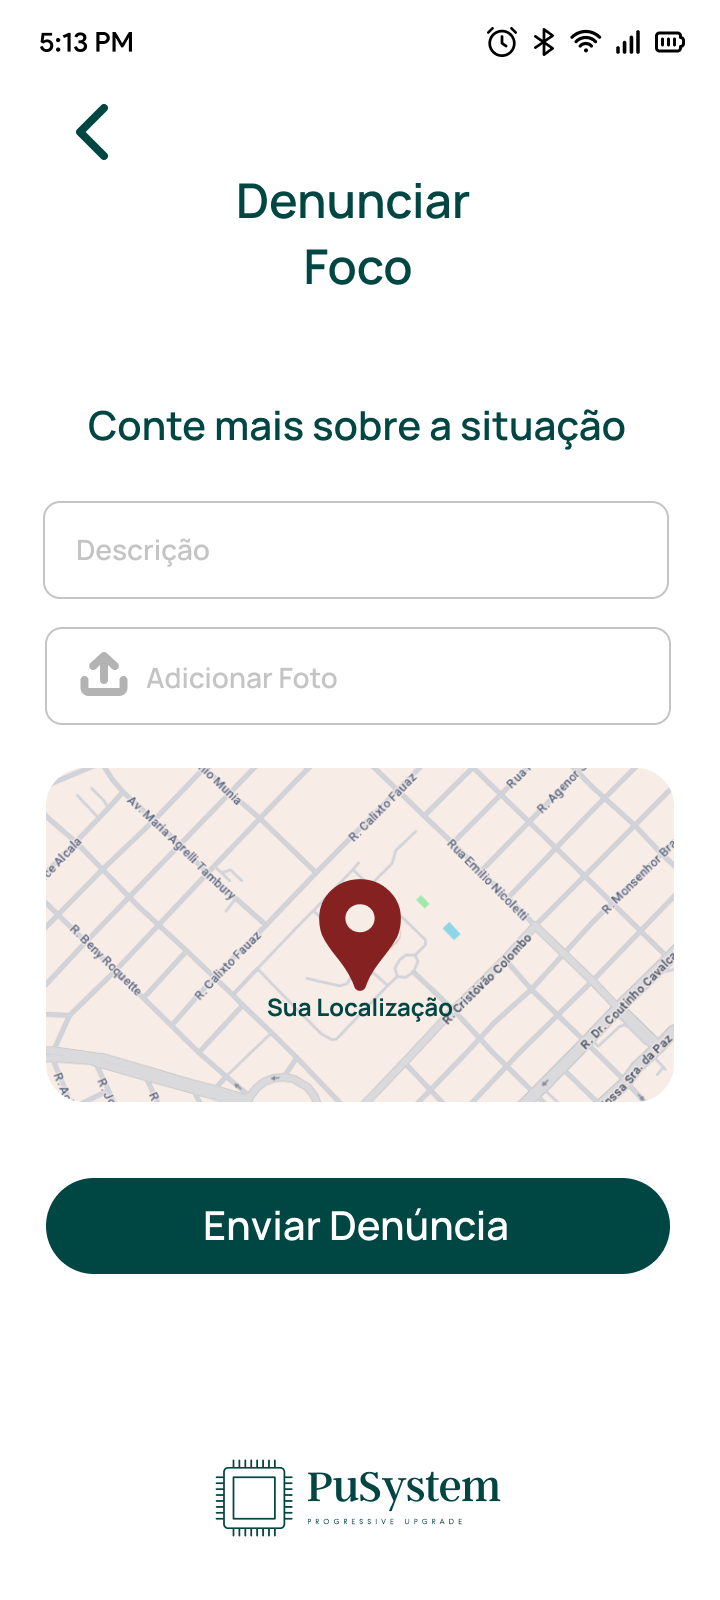
\includegraphics[width=0.5\textwidth]{dist/denunciar-foco.png}}
  \caption{Tela de Denúncias}
  \label{fig:denuncia}
\end{figure}

Na tela de denúncia de focos, a ênfase está na praticidade e exatidão: a localização automática via GPS simplifica o procedimento, porém a possibilidade de ajuste manual assegura flexibilidade em caso de erro.  O envio integrado de imagens reforça a denúncia com provas visuais, e a confirmação de envio com retorno reforça a segurança do usuário de que sua contribuição foi recebida e está sendo tratada.

\subsubsection{Tela Monitoramento de Sintomas}

\begin{figure}[H]
  \centering
  \fbox{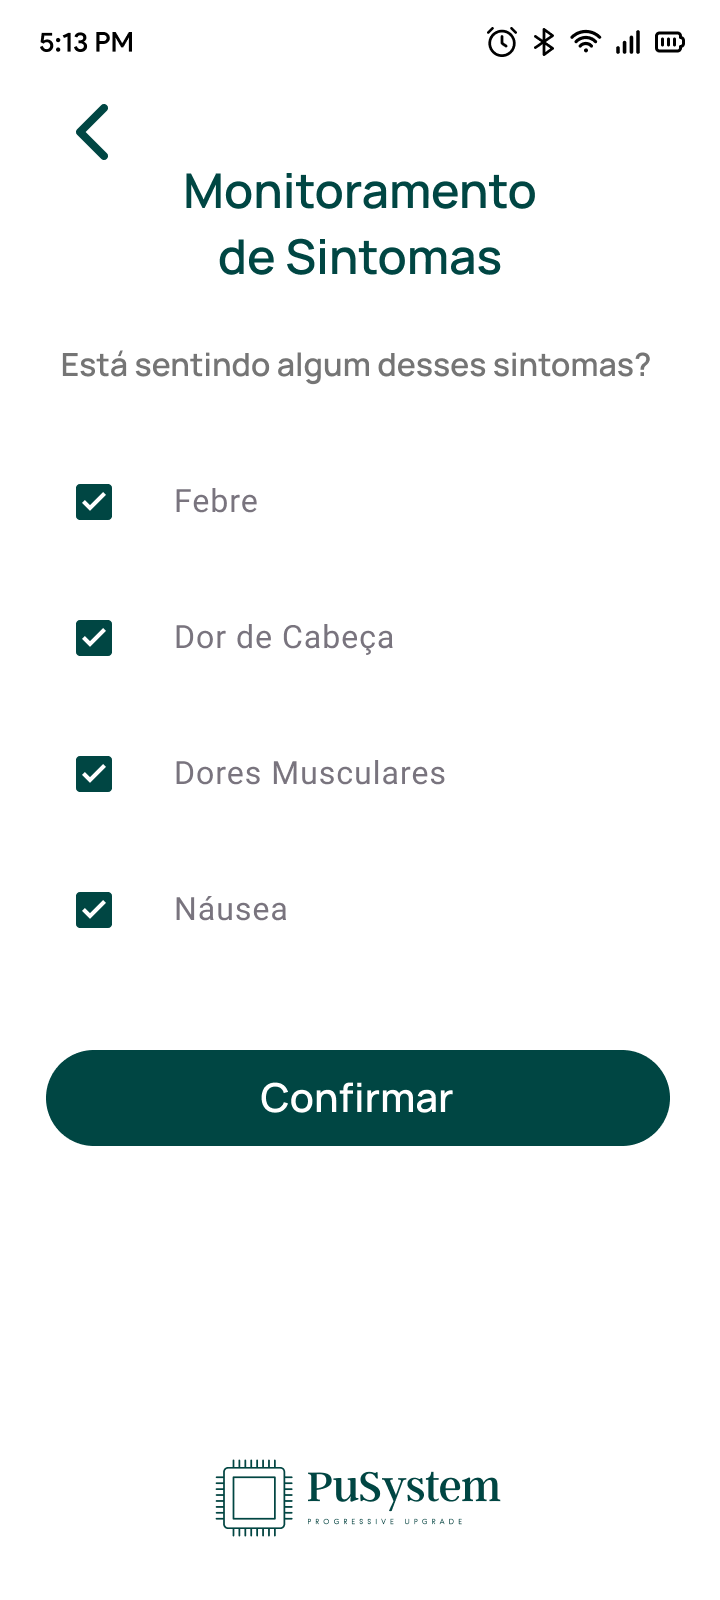
\includegraphics[width=0.5\textwidth]{dist/monitoramento-de-sintomas.png}}
  \caption{Monitoramento de Sintomas}
  \label{fig:sintomas}
\end{figure}

A interface de monitoramento de sintomas possui um checklist intuitivo, onde os sintomas mais frequentes são apresentados de maneira clara, facilitando a escolha do usuário sobre o que está sentindo.  Isso reduz o esforço cognitivo e aprimora a exatidão do relato, crucial para produzir alertas de saúde.

\subsubsection{Tela Aprender}

\begin{figure}[H]
  \centering
  \fbox{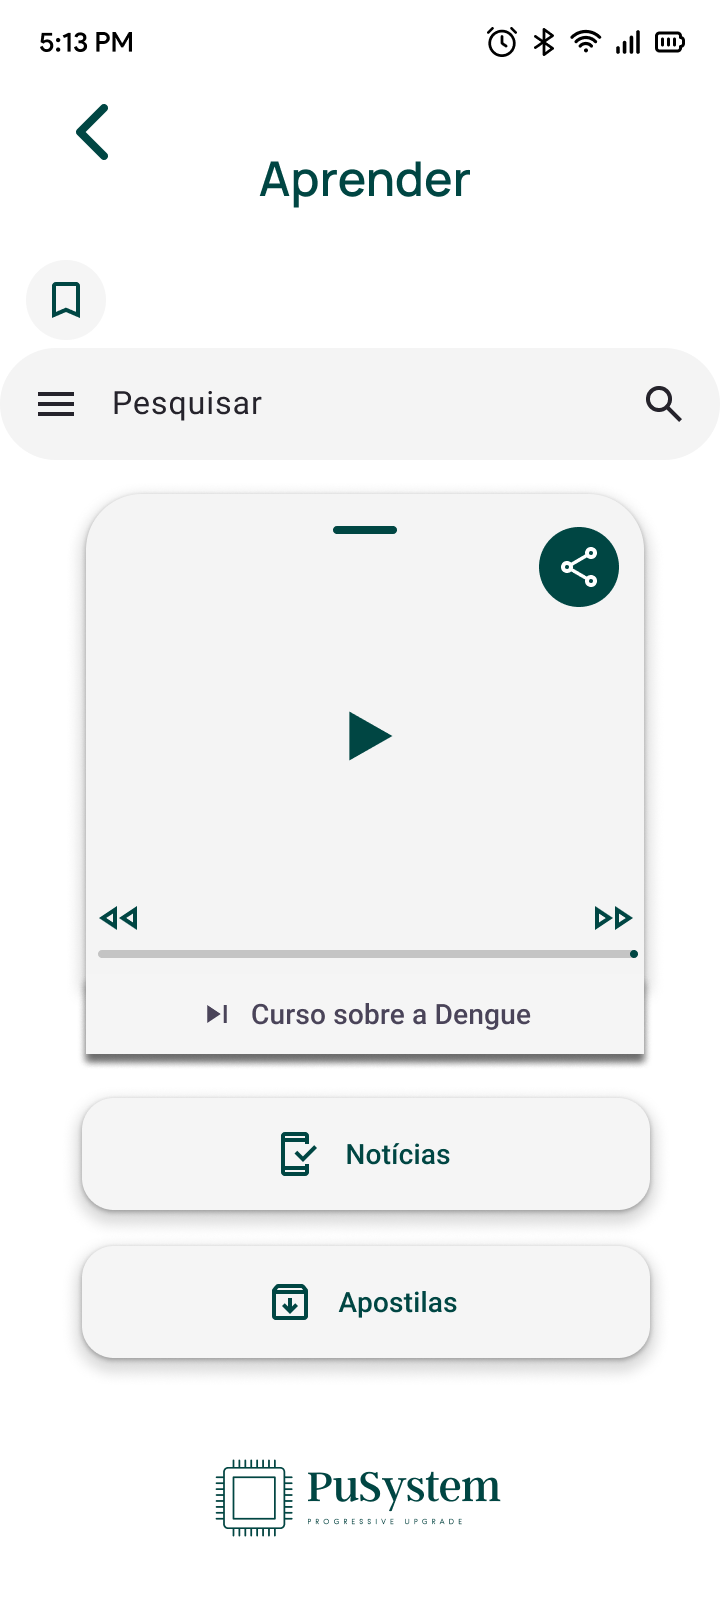
\includegraphics[width=0.5\textwidth]{dist/modulo-educacional.png}}
  \caption{Módulo Educacional}
  \label{fig:educacao}
\end{figure}

Na tela "Aprender", an estrutura foi planejada para potencializar o efeito educativo.  Foram organizados diversos materiais, incluindo vídeos, artigos e apostilas, com ênfase em informações críticas.  A pesquisa por temas e o avanço do aprendizado auxiliam o usuário a percorrer o conteúdo. Por outro lado, os botões de salvar, reproduzir e compartilhar estimulam a propagação do saber e a memorização das informações.

\subsubsection{Tela Missões}

\begin{figure}[H]
  \centering
  \fbox{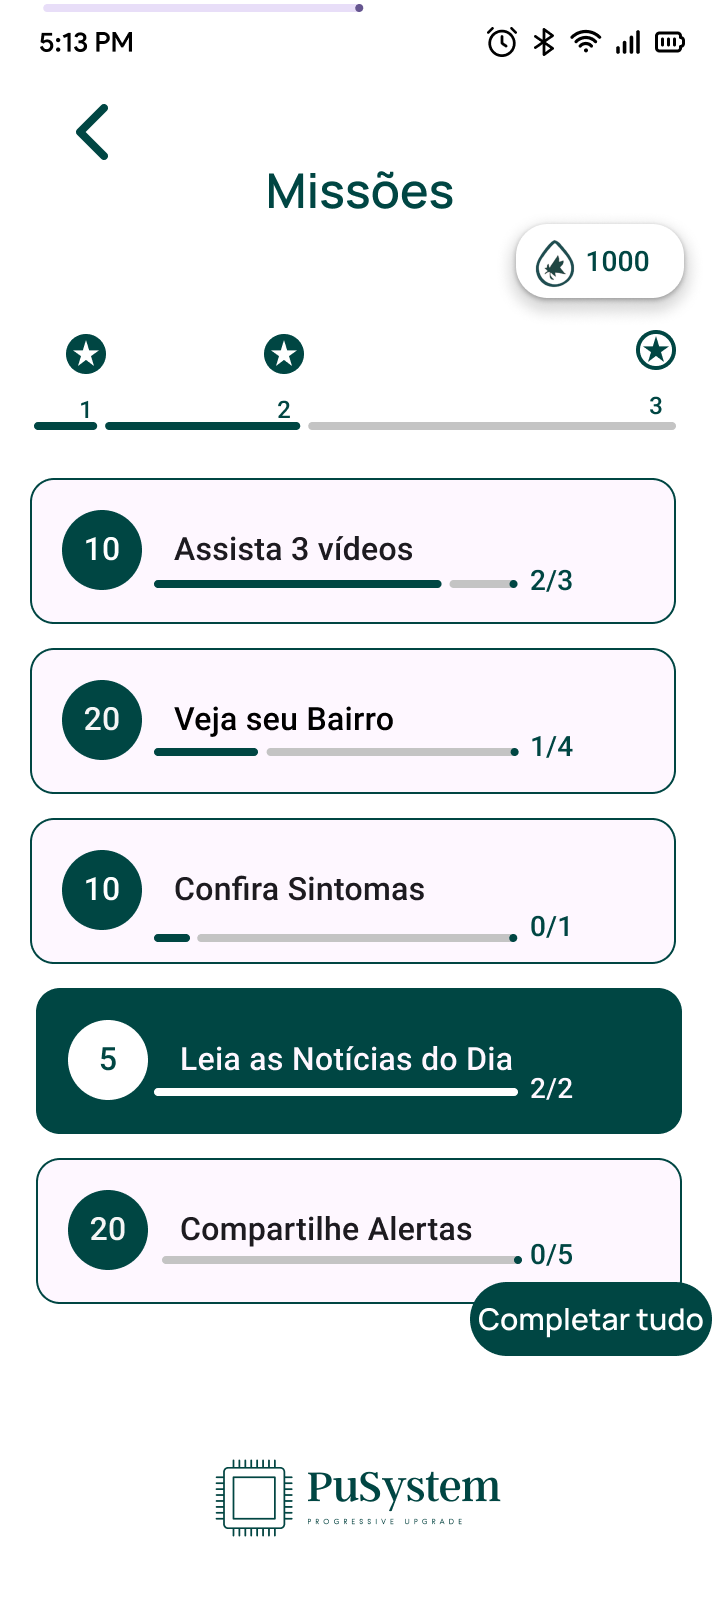
\includegraphics[width=0.5\textwidth]{dist/missoes.png}}
  \caption{Tela de Gamificação}
  \label{fig:missao}
\end{figure}

A interface de missões inclui componentes de gamificação, como o sistema de pontos, prêmios e indicadores de avanço, que contribuem para manter a motivação e incentivar atitudes positivas.  O sistema de conquistas e a pontuação visual proporcionam ao usuário uma sensação contínua de avanço, inclusão e influência na comunidade.

\subsubsection{Tela de Loading}

\begin{figure}[H]
  \centering
  \fbox{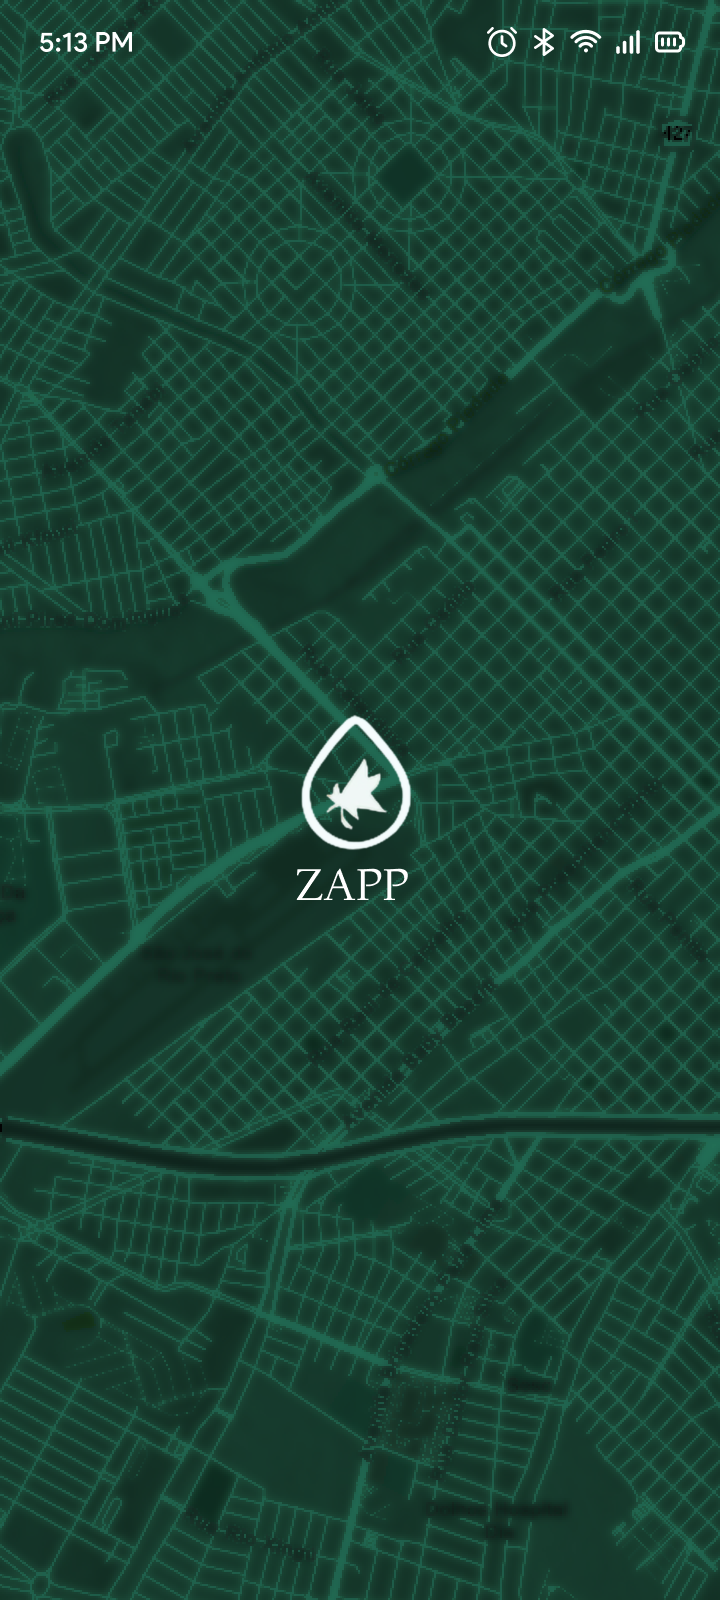
\includegraphics[width=0.5\textwidth]{dist/splash-screen.png}}
  \caption{Splash Screen}
  \label{fig:loading}
\end{figure}

Por fim, a tela de loading não foi negligenciada: ela oferece feedback visual ao usuário por meio de um indicador de carregamento com ícone piscante, evitando a sensação de inatividade ou erro. O mapa de fundo, em verde, reforça a identidade visual do aplicativo, criando uma conexão emocional e estética mesmo nos momentos de espera.

\subsection{Construção}

A elaboração da interface seguirá um processo iterativo, iniciando com a prototipagem em papel para validação inicial das ideias, assegurando rapidez e custo reduzido nas alterações. Posteriormente, serão criados protótipos funcionais, possibilitando testes reais e correções antes da codificação final. 

Ademais, a construção da interface será desenvolvida utilizando frameworks multiplataforma modernos, com ênfase no React Native em combinação com o TypeScript, garantindo compatibilidade integral com dispositivos Android e iOS. A interface priorizará design responsivo, adaptando-se a diferentes tamanhos de tela e orientações (retrato/paisagem). Além disso, foi concebida com foco em acessibilidade, seguindo diretrizes como contraste adequado e navegação simplificada.

Os testes com usuários reais permitirão identificar áreas críticas e validar decisões de design, enquanto o aprimoramento constante com base em \textit{feedback} permitirá aprimorar a interface para atingir o equilíbrio perfeito entre estética, funcionalidade e usabilidade.



\subsection{Validação}

A validação do projeto será feita meticulosamente, aplicando testes de usabilidade para diversos perfis de usuários, assegurando que o sistema atenda desde iniciantes até usuários avançados. Dados quantitativos e qualitativos serão coletados através de questionários, possibilitando uma análise completa do desempenho da interface. Serão feitos ajustes finais com base nesses dados, consolidando um produto que proporcionará uma experiência confiável, eficaz e em consonância com os objetivos do projeto.

\newpage
\section{Conclusão}

O protótipo de interface desenvolvido para o aplicativo Zapp cumpre os objetivos estabelecidos, alinhando os requisitos de usabilidade, acessibilidade e engajamento social. As telas foram projetadas e construídas considerando não apenas a estética visual, mas também a eficiência e a clareza das interações, garantindo que usuários de diferentes perfis possam navegar pelo aplicativo sem dificuldades.  

Além disso, a adoção de práticas de prototipação, testes de usabilidade e validação contínua com usuários reais permitiu refinar a interface de forma iterativa, resultando em um produto final robusto e adaptado às necessidades do público-alvo.  

Acreditamos que o Zapp tem potencial para se tornar uma ferramenta relevante no contexto de saúde pública, unindo tecnologia, educação e participação comunitária para reduzir a incidência de dengue e fortalecer o senso de responsabilidade coletiva.

\newpage
\begin{thebibliography}{09}
\bibitem{pressman-2019} PRESSMAN, R. S. 
\textbf{Engenharia de Software}. 
8. ed. McGraw Hill, 2019.


\bibitem{nielsen} NIELSEN, J. 
\textbf{10 Usability Heuristics for User Interface Design}. 
Nielsen Norman Group, 1994.
\end{thebibliography}

\end{document}
